\lhead{Metodología de desarrollo}
\chapter{Metodología de desarrollo}

\section{Planificación temporal}

% \begin{figure}[H]
% 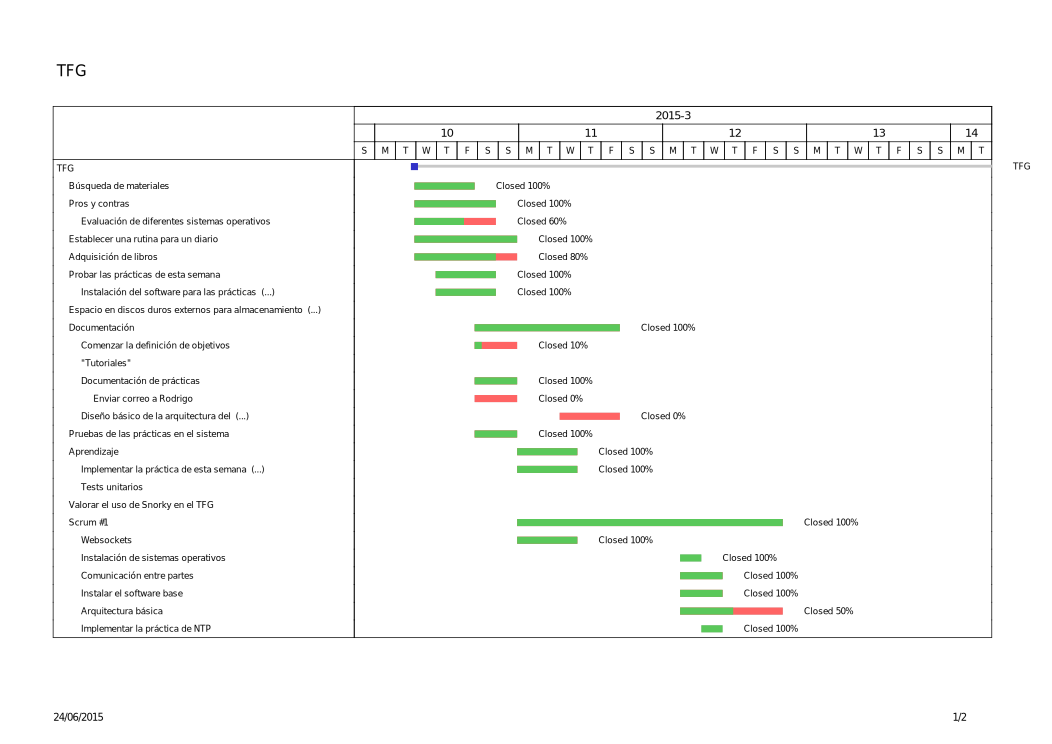
\includepdf[pages=1,pagecommand={},offset=-2.5cm -3cm]{Chapters/Chapter10/Figures/tfg-gantt-mar.pdf}
% \caption{Actividad realizada en el mes de marzo}
% \end{figure}
% \includepdf[pages=2,pagecommand={},offset=-2.5cm -3cm]{Chapters/Chapter10/Figures/tfg-gantt-mar.pdf}
% 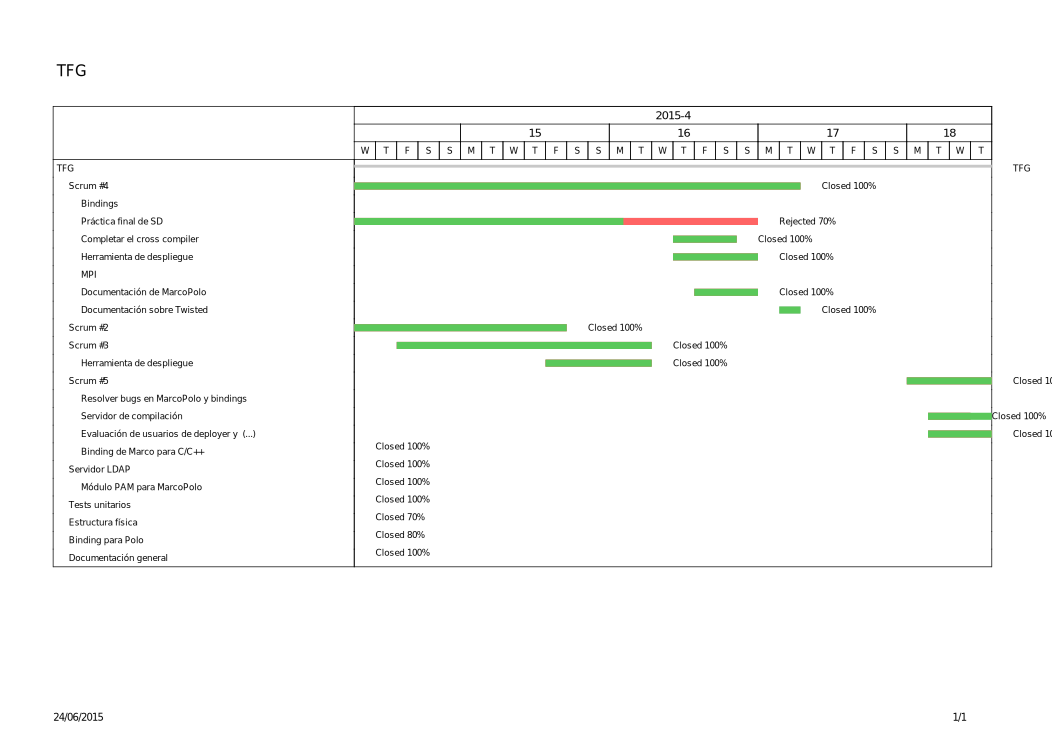
\includepdf[pages=1,pagecommand={},offset=-2.5cm -3cm]{Chapters/Chapter10/Figures/tfg-gantt-apr.pdf}
% 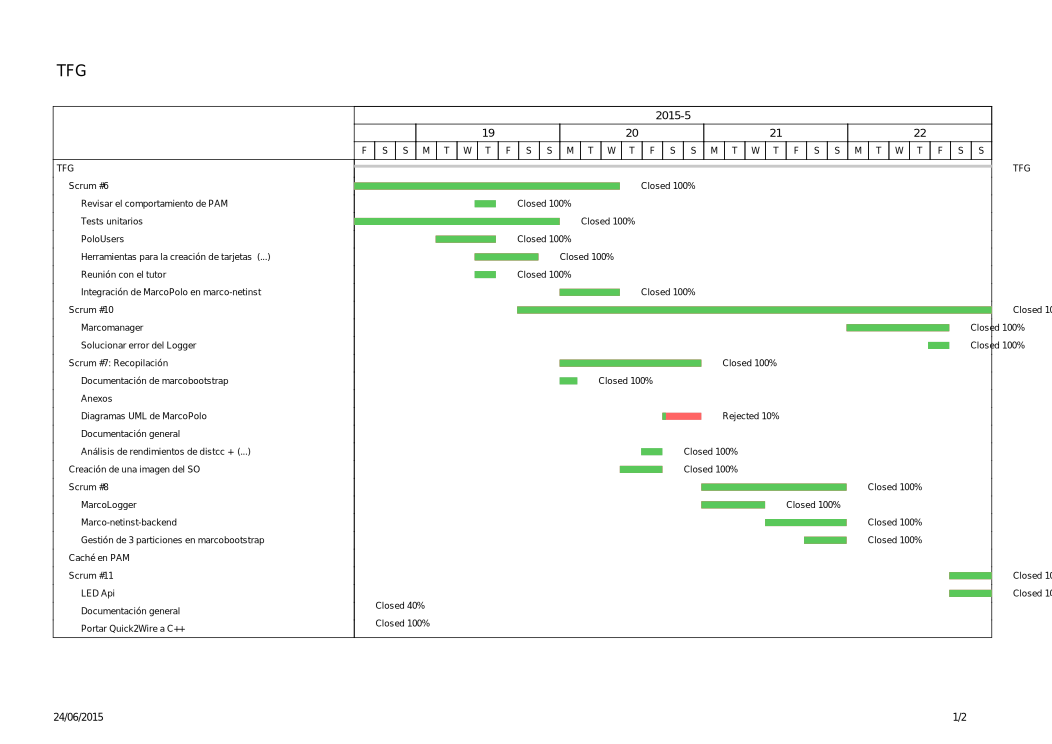
\includepdf[pages=1,pagecommand={},offset=-2.5cm -3cm]{Chapters/Chapter10/Figures/tfg-gantt-may.pdf}
% \includepdf[pages=2,pagecommand={},offset=-2.5cm -3cm]{Chapters/Chapter10/Figures/tfg-gantt-may.pdf}
% 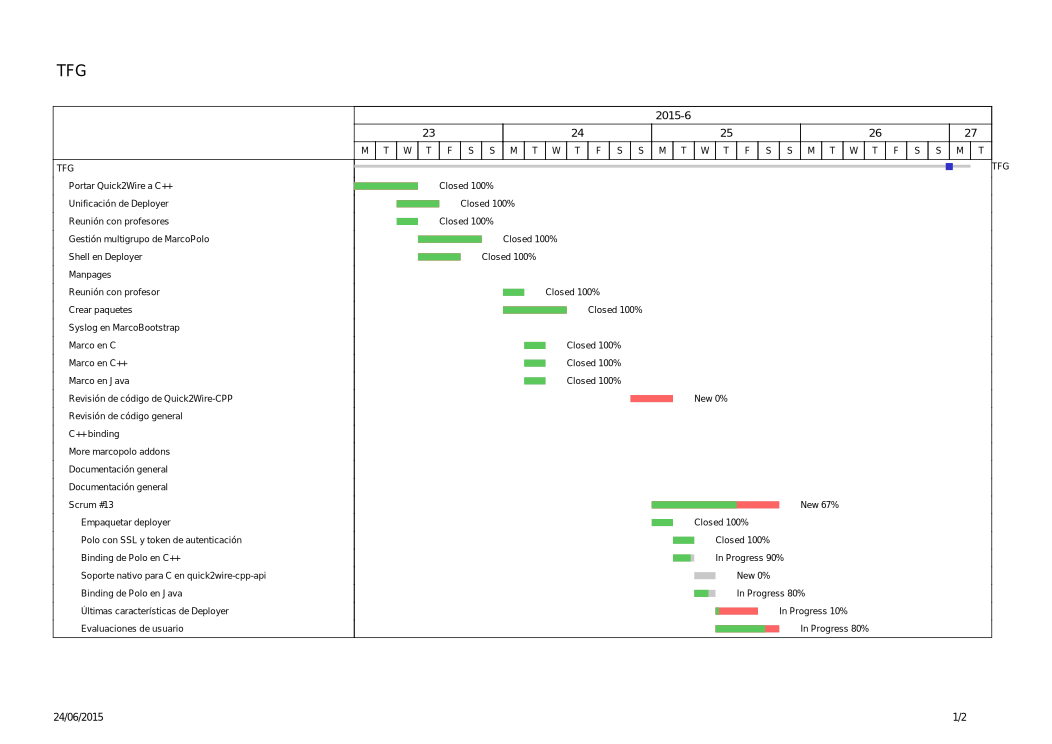
\includepdf[pages=1,pagecommand={},offset=-2.5cm -3cm]{Chapters/Chapter10/Figures/tfg-gantt-jun.pdf}
% \includepdf[pages=2,pagecommand={},offset=-2.5cm -3cm]{Chapters/Chapter10/Figures/tfg-gantt-jun.pdf}
% %\includepdf[pages=2,pagecommand={},offset=-2.5cm -3cm]{Chapters/Chapter10/Figures/tfg-gantt-apr.pdf}

\begin{figure}[H]
\centering
\includegraphics[width=0.7\textwidth]{Chapters/Chapter10/Figures/tfg-gantt-mar}
\end{figure}

\begin{figure}[H]
\centering
\includegraphics[width=0.7\textwidth]{Chapters/Chapter10/Figures/tfg-gantt-apr}
\end{figure}
\begin{figure}[H]
\centering
\includegraphics[width=0.7\textwidth]{Chapters/Chapter10/Figures/tfg-gantt-may}
\end{figure}
\begin{figure}[H]
\centering
\includegraphics[width=0.7\textwidth]{Chapters/Chapter10/Figures/tfg-gantt-jun}
\end{figure}
